\section{Conception \& Architecture}
\subsection{Technologies utilisées}
\subsubsection{Java 8}
Parmi les deux langages de haut niveau proposés pour l'élaboration de ce projet (Java ou C++), nous avons choisi Java pour sa portabilité, sa sécurité et ses performances. De plus, la dernière version de Java propose la librairie graphique JavaFX qui correspond en tout point à notre projet. Enfin, notre équipe est également plus habile à programmer à l'aide du langage Java.

\subsubsection{JavaFX 8}
JavaFX, successeur de Swing, est la librairie de création d'interface graphiques officielle de Java. La version 8, utilisée pour ce projet, ajoute de nouvelles fonctionnalités et est la plus récente version utilisable avec Scene Builder.

\begin{figure}[h]
    \caption{Architecture de JavaFX}
    \centering
    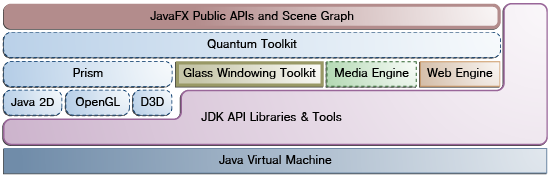
\includegraphics[width=\textwidth]{arch_javafx.png}
    \label{fig:arch_javafx}
\end{figure}

Comme vous pouvez le voir sur la figure \ref{fig:arch_javafx}, BLA BLA BLA A COMPLETER, A PARLER DE CSS ETC


\subsubsection{Scene Builder 8.3.0}
Scene Builder de Gluon permet de manipuler des objets JavaFX graphiquement et exporter ceux-ci dans un fichier .fxml interprétable par la librairie graphique. L'interface de base à été conçue lors de l'élaboration du cahier des charges pour présenter un exemple de l'interface de l'application finale. Plusieurs mock-ups ont été présentés et c'est sur ceux-cis que nous nous sommes basés pour construire, grâce à Scene Builder, une base d'interface sur la laquelle nous avons rajouté des composants et fonctionnalités tout au long de l'élaboration de l'application. La flexibilité de JavaFX permet d'ajouter des éléments via un fichier externe fxml mais aussi directement dans le code, ce que nous avons aussi utilisé.

\subsubsection{Maven}
Pour la compilation du projet et l'importation aisée de celui-ci dans un nouvel environnement de travail, nous avons utilisé l'outil Maven de Apache.
TODO TODO TODO TODO TODO COMPLETER

\subsubsection{Git}
Git est un logiciel de gestion de version utilisé pour permettre de stocker tous les fichiers du projet ainsi que toutes les modifications leur ayant été apportés depuis leur création. Pour chaque nouvelle fonctionnalité, nous avons procédé par la création d'une branche à partir de la branche principale (une version fonctionnelle du programme, contenant les fonctionnalités implémentées et testées). Ces nouvelles branches permettent de développer les fonctionnalités du programme indépendamment et de les ajouter à la branche principale une fois inspectées et testées par plusieurs membres de l'équipe.

\subsubsection{GitHub}
Github est un service web permettant de parcourir visuellement l'historique Git ainsi que de fournir des outils de gestion de Git. Notamment, pour chaque fonctionnalité ou chaque bug découvert, une "issue" (un problème) peut être ouverte et assignée à un ou plusieurs membres de l'équipe. Dès la fin de l'élaboration du planning de notre projet, des issues ont été assignées à chaque développeur. Celles-ci ont permis de mieux se fier au planning et toujours avoir en vue ce qu'il restait à implémenter.

\subsection{Comparaison de l'interface finale avec notre mock-up}
TODO TODO TODO TODO TODO Comparer les deux avec une image et parler un peu des changements éventuels